\chapter{System monitorowania Icinga}
\label{chap:Icinga}

W~rozdziale \ref{chap:Systemy} została przeprowadzona analiza
dostępnych na ryku systemów monitorowania. Na jej podstawie dokonano
wyboru systemu Icinga jako podstawy do budowy systemu uwzględniającego
wymagania dotyczące klienta mobilnego. Przed przystąpieniem do
projektowania takiego systemu należy dokładnie zapoznać się
z~możliwościami jak i~ograniczeniami systemu Icinga. W~dalszej części
tego rozdziału przedstawiono w~pełni funkcjonalną konfigurację systemu
monitorowania klientów statycznych. Uwzględniono w~niej nie tylko
system, lecz także dodatki, które będą dla większości konfiguracji
niezbędne. W~ramach tej konfiguracji uwzględniono również potrzebę
analizy zgromadzonych danych. W~proponowanym systemie do tego celu
użyto dodatku {\em inGraph}. W~odróżnieniu od innych dodatków tego typu,
wykorzystuje on relacyjną bazę danych, przez co możliwe jest zarówno
dynamiczne zarządzanie czasem przechowywania danych, jak
i~synchronizacja danych z~okresów w~przeszłości.

W pierwszej części tego rozdziału opisano poszczególne komponenty,
które zostaną wykorzystane w~systemie. Druga część tego rozdziału
prezentuje proponowaną konfigurację przeznaczoną do monitorowania
pojedynczego segmentu sieci. Ponadto przedstawiono możliwości
współpracy wielu instancji rdzenia monitorującego podczas
monitorowania sieci wielosegmentowej. Konfiguracje te mogą zostać
wykorzystane w~rozbudowanych sieciach dużych firm
i~korporacji. Poznanie schematów współpracy wielu rdzeni
monitorujących jest kluczowe dla wykonania prawidłowego projektu
systemu rozproszonego.

\section[Rdzeń monitorujący][Rdzeń monitorujący]{Rdzeń monitorujący}
\label{sec:IcingaCore}

System {\em Icinga} powstał jako klon systemu Nagios. Wprowadzono wiele
poprawek i~zmian architektonicznych jednak zasada funkcjonowania
rdzenia pozostała niezmieniona. W~celu zrozumienia architektury całego
systemu, konieczne jest zapoznanie się z~jego głównym elementem czyli
rdzeniem monitorującym. Jego architektura została przedstawiona na
rys.~\ref{fig:icingaCoreArch}. Jest to centralne miejsce w~którym
wykonuje się przetwarzanie danych o~urządzeniach i~usługach. Dane,
które mają być przetworzone mogą zostać dostarczone na dwa sposoby.

\begin{figure}[ht]
  \caption{Schemat architektury rdzenia monitorującego systemu
    Icinga.}
  \label{fig:icingaCoreArch}
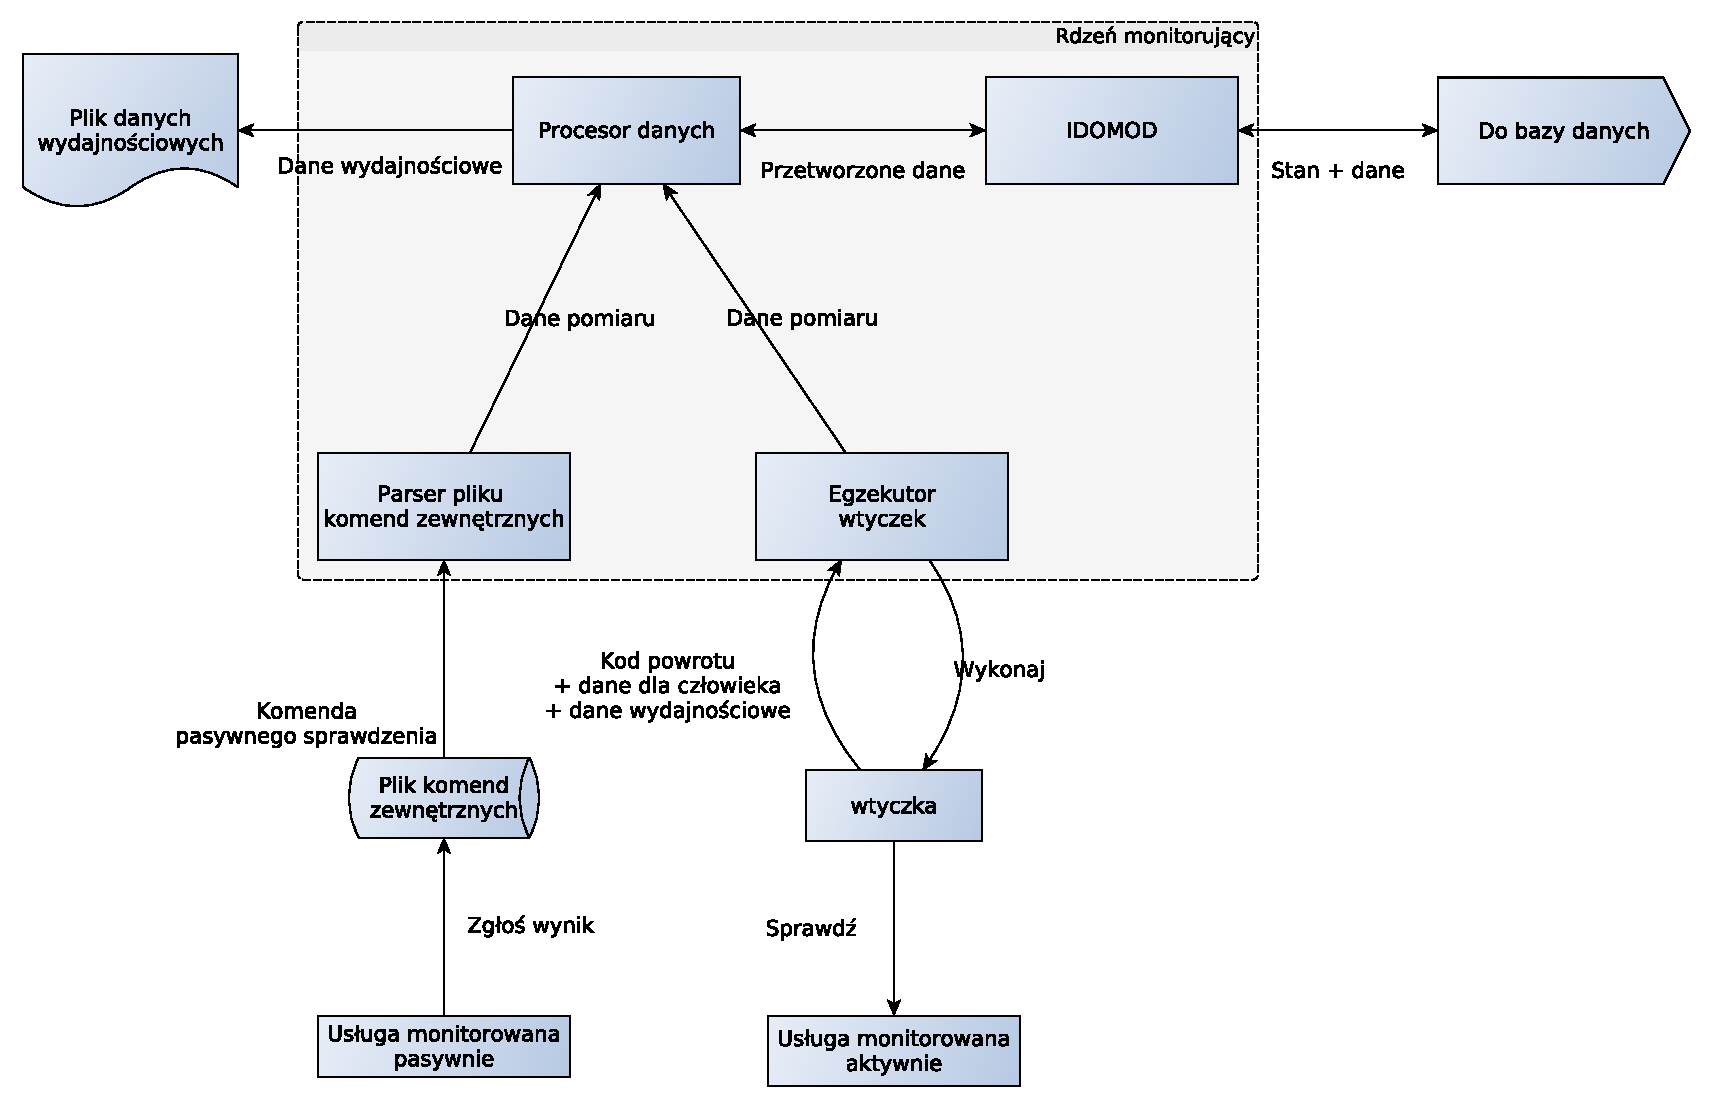
\includegraphics[width=1\textwidth]{img/icingaCoreArch}
\end{figure}


Podstawowy sposób dostarczania danych do przetworzenia opiera się na
monitorowaniu aktywnym. W~systemie {\em Icinga} monitorowanie aktywne odbywa
się poprzez uruchamianie w~określonych odstępach czasowych komend
zdefiniowanych przez użytkownika w~pliku konfiguracyjnym. Standardowa
komenda sprowadza się do uruchomienia wybranego przez administratora
programu (tzw. wtyczki) z~odpowiednimi parametrami. W~ramach wykonania
komendy uruchomiony może zostać dowolny program lub skrypt. Aby jednak
zapewnić poprawne funkcjonowanie całego systemu, niezbędne jest
napisanie programu w~zgodności z~regułami opisanymi
w~\cite{www:NagiosPluginsTutorial}. Reguły te definiują jakie dane
i~w~jaki sposób powinny być przekazane z~programu (wtyczki) do rdzenia
systemu monitorującego. Pierwszym elementem przekazu danych jest
zwrócenie przez wtyczkę odpowiedniego kodu zakończenia
programu. Poszczególne wartości zwrócone mają następujące znaczenie
dla rdzenia monitorującego:

\begin{description}
\item[0] --- OK, wtyczka mogła wykonać sprawdzenie i~usługa lub urządzenie
  jest w~stanie OK.
\item[1] --- WARNING, wtyczka mogła wykonać sprawdzenie, ale parametry
  urządzenia lub usługi przekraczają poziom ostrzegawczy.
\item[2] --- CRITICAL, wtyczka mogła wykonać sprawdzenia ale parametry
  urządzenia lub usługi przekraczają poziom krytyczny.
\item[3] --- UNKNOWN, wtyczka nie była w~stanie wykonać sprawdzenia ze
  względu na dostarczenie nieprawidłowych parametrów wywołania lub
  niskopoziomowego błędu systemu.
\end{description}

Każda wtyczka, poza numerycznym kodem wyjścia z~programu, może
przekazać do rdzenia monitorującego dane w~postaci tekstowej. Minimum
powinna zostać przekazana jedna linia tekstu, natomiast maksymalna
jego długość wynosi 8KB. Dane te powinny być wypisane na standardowe
wyjście wtyczki. Składają się one z~dwóch części. Część przed
znakiem~| (kod ASCII 0x7C) stanowi czytelny dla człowieka opis stanu parametru badanego
przez wtyczkę. Część znajdująca się po tym znaku to tak zwane dane
wydajnościowe (ang. {\em performance data}). Powinny być one
przekazane w~formacie klucz~=~wartość gdyż są przeznaczona do dalszej
obróbki przez zewnętrzne programy np. do generacji
wykresów. Przekazanie danych wydajnościowych nie jest obowiązkowe.

Warto nadmienić, iż wszystkie wtyczki uruchamiane przez rdzeń
monitorujący wykonują się w~kontekście systemu, na którym uruchomiony
jest rdzeń monitorujący. W~celu wykonywania w~sposób aktywny sprawdzeń
parametrów innych urządzeń, konieczne jest użycie mechanizmu, który
pozwoli na uruchamianie wtyczek na zdalnej maszynie. Przykładem
takiego dodatku jest {\em NRPE} omówiony już w~rozdziale~\ref{sec:Nagios}.

Drugą dostępną metodą dostarczenia danych w~celu przetworzenia ich
przez rdzeń monitorujący jest tzw. plik komend zewnętrznych (patrz
rys.\ref{fig:icingaCoreArch}). Pozwala on na monitorowanie usług
w~sposób pasywny. Nie jest to tak na prawdę plik lecz potok
nazwany. W~rdzeniu monitorującym obecny jest element, który
odpowiedzialny jest za czytanie danych z~potoku. Do potoku mogą być
natomiast zapisywane dowolne spośród komend przedstawionych
w~\cite[412-436]{www:IcingaDoc}. Rdzeń monitorujący po przeczytaniu
każdej komendy wykona akcję z~nią powiązaną. Szczególnym przypadkiem
komendy jest żądanie przetworzenia pasywnego sprawdzenia danej usługi
lub urządzenia. Dokładny format tej komendy został opisany
w~\cite[296-299]{www:IcingaDoc}. Należy zwrócić uwagę na dodatkowe,
w~stosunku do sprawdzenia aktywnego, pola. Pierwsze z~pól to stempel
czasu, kiedy zostało wykonane dane sprawdzenie. Kolejne dwie dodatkowe
wartości, czyli nazwa urządzenia oraz usługi, konieczne są w~celu
poprawnej identyfikacji usługi, której dotyczą przekazywane
dane. Reszta komendy zawiera dane o~znaczeniu znanym już
z~monitorowania aktywnego.

Wykonanie zapisu do potoku nazwanego należącego do procesu rdzenia
monitorującego wymaga, aby program, który chce to zrobić, uruchomiony
był na tym samym systemie co rdzeń. Aby umożliwić przekazywanie tych
danych z~innych urządzeń opracowany został dodatek {\em NSCA} dystrybuowany
jako dodatek do systemów Nagios oraz {\em Icinga}. Specyfikuje on protokół
komunikacyjny, który pozwala na przekazanie z~innego systemu do
rdzenia monitorującego wiadomości zawierającej wynik
sprawdzenia. Program ten został szeroko opisany
w~rozdz.~\ref{sec:NSCA}.

Otrzymane w~ten sposób dane są w~kolejnym etapie przetwarzane przez
rdzeń sprawdzający niezależnie od sposobu ich dostarczenia (patrz
rys.~\ref{fig:icingaCoreArch}). Pierwszym etapem przetwarzania tych
danych jest wydzielenie z~nich danych przeznaczonych dla człowieka
oraz danych wydajnościowych przeznaczonych do przetwarzania przez inne
dodatki. Dane wydajnościowe zawierają wyniki pomiarów przeprowadzonych
przez wtyczkę w~trakcie determinowania jej stanu. Po wydzieleniu
zostają one udostępnione na zewnątrz rdzenia monitorującego poprzez
pliki tekstowe o~zadanym w~konfiguracji formacie. Dane te są
wykorzystywane przez dodatki przeznaczone do generacji wykresów takie
jak opisany w~rozdz.~\ref{sec:inGraph} dodatek {\em inGraph}. Poza eksportem
danych wydajnościowych, w~ramach przetwarzania dokonywane jest
wyznaczenie stanu usługi na podstawie danych poprzednich oraz nowo
dostarczonych. Po wykonaniu całego niezbędnego przetwarzania wszystkie
dane otrzymane od wtyczki są przekazywane do modułu rdzenia IDOMOD,
będącego częścią komponentu {\em IDOUtils}. Komponent ten pozwala na
przechowywanie danych operacyjnych systemu monitorującego w~bazie
danych. Został on szczegółowo opisany w~rozdz.~~\ref{sec:IDOUtils}.

\section[Komponent IDOUtils][Komponent IDOUtils]{Komponent IDOUtils}
\label{sec:IDOUtils}

Komponent {\em IDOUtils} czyli {\em Icinga Database Object Utilities} jest
to zestaw programów, dzięki którym możliwe jest składowanie w~bazie
danych informacji generowanych przez rdzeń monitorujący. W~wersji
dostępnej podczas pisania tej pracy wspierane były następujące systemy
zarządzania bazą danych:

\begin{itemize}
\item MySql,
\item PostgreSQL,
\item Oracle.
\end{itemize}

W~celu zapewnienia funkcjonalności omawianego komponentu, konieczne
jest utworzenie bazy danych o~odpowiednim schemacie, który został
opisany w~\cite[669-750]{www:IcingaDoc}. Udostępnione zostały również
skrypty SQL, które definiują wymagane tabele. Ponadto administrator
musi zapewnić odpowiednią konfigurację bazy danych, w~tym konto
użytkownika i~hasło w~taki sposób, aby umożliwić odpowiednim
elementom komponentu {\em IDOUtils} dostęp do bazy danych.

W~celu odciążenia komputera, na którym uruchomiony jest rdzeń systemu
{\em Icinga}, komponent ten został podzielony na kilka elementów, które mogą
znajdować się na różnych systemach. Można wyróżnić następujące
elementy:

\begin{description}
\item[IDOMOD] --- moduł rdzenia monitorującego, który pozwala mu na dostęp
  do bazy danych.
\item[LOG2IDO] --- program pozwalający na import utworzonych wcześniej
  plików do bazy danych.
\item[FILE2SOCK] --- program pozwalający na przekierowanie danych
  zapisywanych do pliku do gniazda TCP lub Unix.
\item[IDO2DB] --- demon, który jest odpowiedzialny za wykonywanie operacji
  na bazie danych.
\end{description}

\begin{figure}[ht]
  \caption{Schemat integracji IDOUtils z systemem Icinga.}
  \label{fig:IDOUtilsArch}
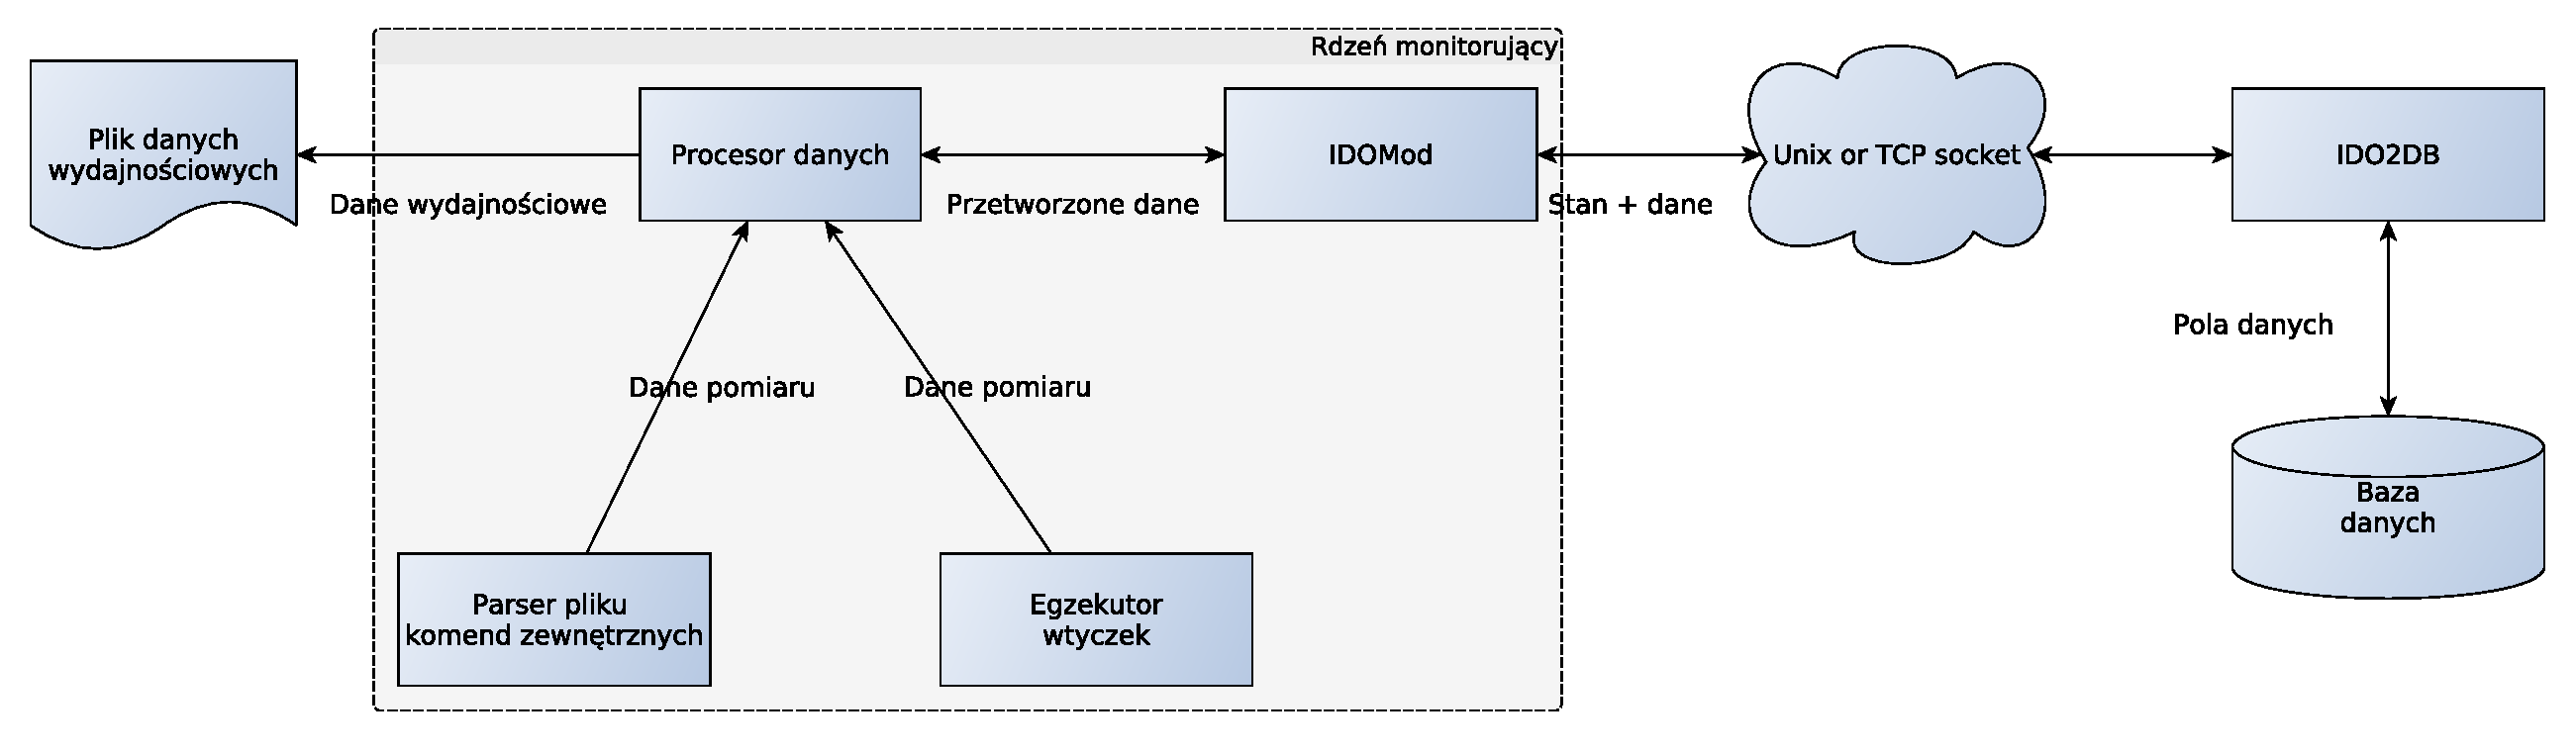
\includegraphics[width=1\textwidth]{img/idoutilsArch}
\end{figure}

Podstawowymi elementami całego komponentu są IDOMOD oraz
IDO2DB. Schemat ich typowego zastosowania przedstawiono na
rys.~\ref{fig:IDOUtilsArch}. Moduł rdzenia IDOMOD ładowany jest przez
rdzeń systemu {\em Icinga} tuż po starcie. Po załadowaniu zapewnia on spójny
interfejs do uzyskiwania danych dla wszystkich pozostałych części
rdzenia monitorującego. Ponieważ wykonywanie operacji na bazie danych
może być czasochłonne, nie powinno być wykonywane przez rdzeń
monitorujący. Z~tego powodu powstał program IDO2DB. Jest on
uruchomiony jako demon na dowolnym urządzeniu. Zadaniem tego serwisu
jest fizyczna realizacja żądań na bazie danych. Na schemacie celowo
pominięto pozostałe elementy tego komponentu, gdyż stanowią one
jedynie inne źródło danych dla demona IDO2DB i~są konieczne jedynie
przy imporcie danych historycznych ze~starej instalacji systemu, lub
bardziej zaawansowanych konfiguracjach.

Ponieważ rdzeń monitorujący oraz demon IDO2DB mogą znajdować się
zarówno na jednym komputerze, jak i~na różnych konieczne jest
zapewnienie odpowiednich mechanizmów komunikacji pomiędzy nimi.  Gdy
programy te znajdują się na różnych systemach, jako mechanizm
komunikacji wykorzystywane są gniazda TCP. W~podstawowej konfiguracji
dane przekazywane są w~sposób niezaszyfrowany. Jeśli jednak istnieje
potrzeba zapewnienia tajności oraz integralności przekazywanych
danych, możliwe jest użycie protokołu SSL\footnote{ ang. {\em Secure
    Socket Layer} -- protokół warstwy prezentacji, zapewniający
  poufność oraz integralność przesyłanych danych.}. W~sytuacji gdy oba
programy uruchomione są na tym samym urządzeniu, w~celu poprawy
wydajności możliwe jest użycie gniazd protokołu Unix\footnote{
  ang. {\em Unix Domain Socket} -- metoda komunikacji międzyprocesowej
  w~systemach Unix. Posiada jednolite API, jak gniazda domeny
  internetowej.}.

Program IDO2DB jest bardzo elastyczny. Nie posiada on ograniczenia co
do liczby podłączonych do niego modułów IDOMOD czy innych
elementów. Pozwala to na wykorzystanie wspólnej bazy danych przez
wiele instancji rdzenia monitorującego. Opisana konstrukcja została
schematycznie przedstawiona na~rys.~\ref{fig:IDOUtils}. Warto
zaznaczyć, że interfejs graficzny icinga-web jest również kompatybilny
z~tym rozwiązaniem. Pozwala to na wyświetlanie w~jednym interfejsie
danych pochodzących od wielu rdzeni monitorujących.

\begin{figure}[ht]
  \caption{Schemat wykorzystania IDOUtils w~systemie Icinga.}
  \label{fig:IDOUtils}
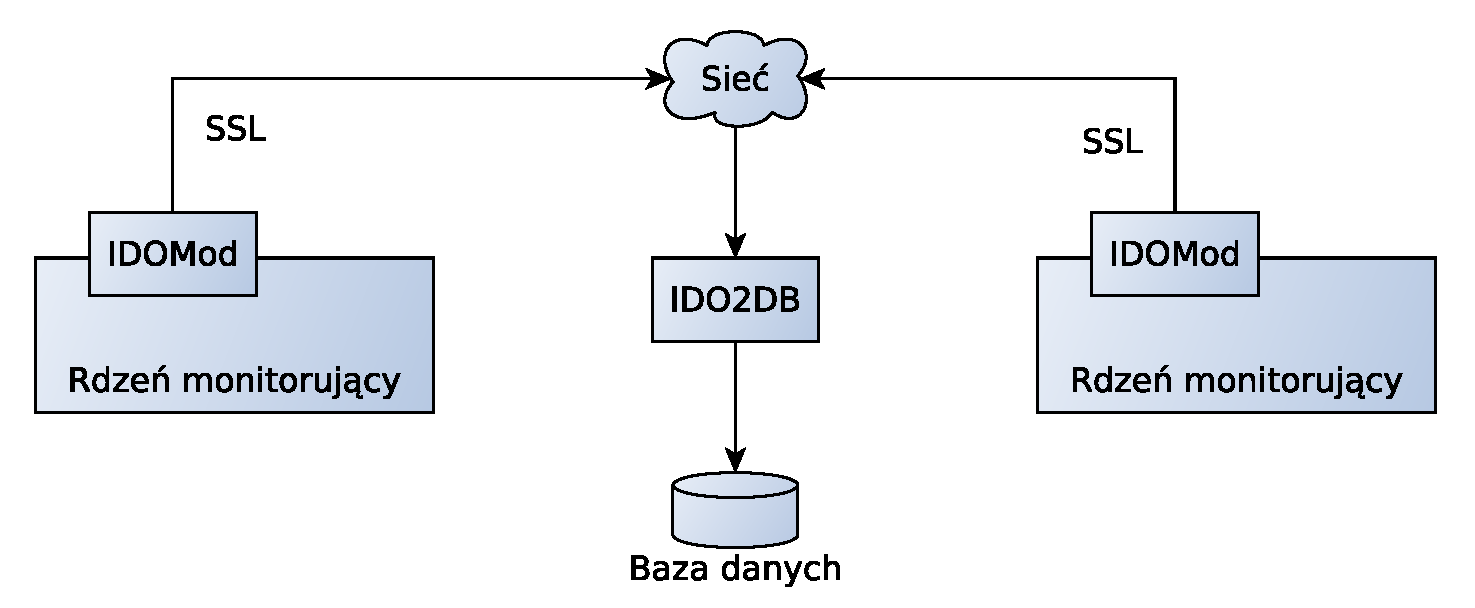
\includegraphics[width=1\textwidth]{img/idoutils}
\end{figure}

W~celu zapewnienia możliwości migracji ze~środowiska, które korzystało
wcześniej z~przechowywania danych w~plikach, został dostarczony
program LOG2IDO. Pozwala on na import danych historycznych do bazy
danych. Program ten, analogicznie jak IDOMOD, nie operuje bezpośrednio
na bazie danych, lecz komunikuje się tymi samymi metodami, co IDOMOD
z~demonem IDO2DB. Zarówno program LOG2IDO, jak i~moduł IDOMOD mogą
kierować żądania do IDO2DB poprzez plik. Aby umożliwić przekazywanie
tych danych z~pliku do demona IDO2DB, opracowano program
FILE2SOCK. Jest to prosty program, który przekazuje dane zapisane do
danego pliku do demona IDO2DB. Program ten nie zajmuje się w~żadnym
stopniu przetwarzaniem odczytaniem danych, lecz jedynie przesłaniem
ich poprzez gniazdo internetowe lub Unix do demona IDO2DB.

\section[Dodatek inGraph][Dodatek inGraph]{Dodatek inGraph}
\label{sec:inGraph}

{\em inGraph} jest dodatkiem do systemów {\em Icinga} oraz Nagios, który umożliwia
prezentację danych zgromadzonych poprzez system monitorujący w~postaci
wykresów. Dodatek ten został opracowany przez firmę NETWAYS GmbH
i~wydany na licencji GPL w~wersji 3. Cechą, która odróżnia dodatek
{\em inGraph} od innych rozwiązań przeznaczonych do analizy danych
historycznych jest wykorzystanie relacyjnej bazy danych do
przechowywania danych otrzymanych od systemu monitorującego. Należy
podkreślić, ze ten dodatek funkcjonuje jako zupełnie odzielny
program. Posiada on ponadto własną, niezalezną bazę danych. Jedynym
punktem integracji tego dodatku z~systemem {\em Icinga} jest wspólny
interfejs graficzny.  Na podstawie otrzymanych danych dodatek {\em inGraph}
dokonuje przeliczeń dla odpowiednich przedziałów czasowych, które
używane są do późniejszej generacji wykresów. Rozmiary przedziałów
definiowane są przez użytkownika w~plikach
konfiguracyjnych. Wykorzystanie tego rodzaju bazy danych powoduje
nieustanny wzrost rozmiaru bazy. W~celu optymalizacji zajętości
przestrzeni dyskowej dodatek {\em inGraph} administruje danymi zgodnie
z~polityką, która również jest definiowana w~jego plikach
konfiguracyjnych. Dla każdego przedziału czasowego zdefiniowany jest
również okres przechowywania danych. Dodatek umożliwia przeglądanie
danych dokładnych z~najmniejszych przedziałów czasu oraz wykresów
długoterminowych prezentujących trendy danej wartości. Ponieważ dane
są bezpośrednio administrowane przez dodatek {\em inGraph}, możliwa jest
zmiana czasu przechowywania danych z~wskazanych przedziałów nawet
w~trakcie działania systemu\footnote{Dla porównania należy przypomnieć
  systemy oparte na cyklicznych bazach danych, w~których rozmiar
  definiowany może być tylko i wyłącznie podczas tworzenia bazy.}.

Dodatek {\em inGraph} składa się z~dwóch niezależnych elementów,
komunikujących się poprzez XML-RPC\footnote{ang. {\em XML Remote
    Procedure Call} --- zdalne wywołanie procedur przy użyciu
  XML. Metoda zdalnego wywoływania funkcji oparta na dokumentach w
  formacie XML. Szczegółowy opis w~\cite{www:XMLRPC}.}:

\begin{description}
\item[ingraph] interfejs graficzny,
\item[ingraph-collector] program zbierający dane.
\end{description}

\begin{figure}[ht]
  \caption{Typowy przepływ danych przy wykorzystaniu dodatku inGraph.}
  \label{fig:inGraphFlow}
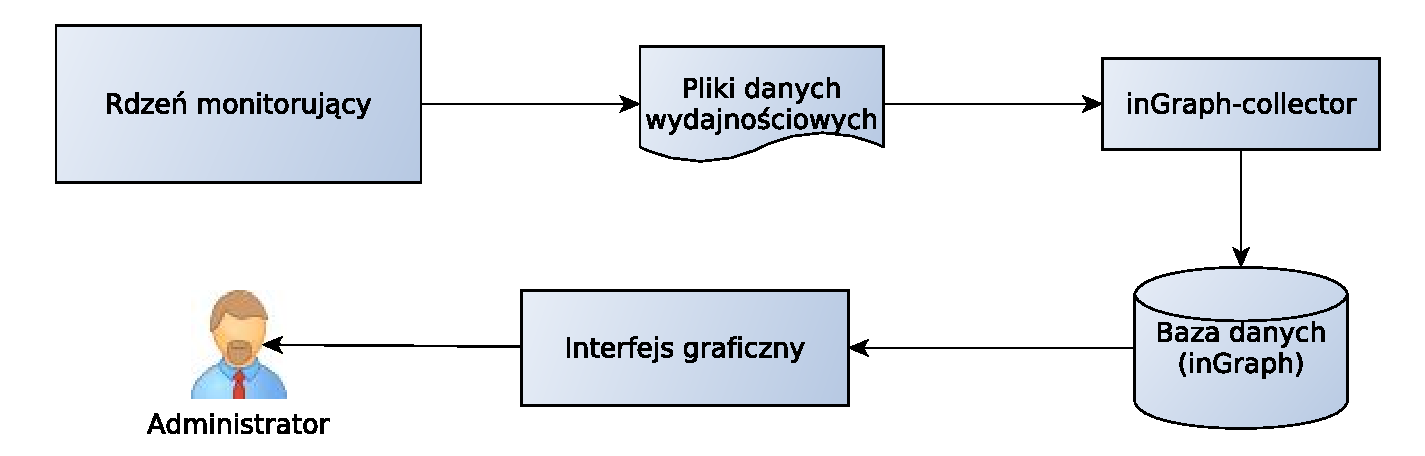
\includegraphics[width=1\textwidth]{img/ingraphFlow}
\end{figure}

Program zbierający oraz przetwarzający dane został napisany w~języku
Python i~nosi nazwę {\em ingraph-collector}. Jego zadaniem jest pobieranie
danych od systemu monitorującego, dokonywanie ich przeliczeń oraz
umieszczanie ich wyników w~bazie danych.

Do pobierania danych z~systemu monitorującego wykorzystano mechanizm
udostępniania danych wydajnościowych. Oznacza to, że rdzeń systemu
monitorującego przekazuje dane wydajnościowe otrzymane od wtyczek
poprzez plik tekstowy. Oczywiście dane muszą być eksportowane przy
pomocy formatu zrozumiałego dla dodatku {\em inGraph}. Demon
{\em ingraph-collector} wykonuje ich analizę, a~następnie wykonuje wszystkie
niezbędne obliczenia np. średnich wartości w~zadanych przedziałach
czasowych. Wyniki zapisywane są w~bazie danych MySQL lub PostgreSQL
programu {\em inGraph}. Należy zwrócić uwagę, iż jest to inna baza danych,
niż ta z~której korzysta system {\em Icinga}. Ważną różnicą pomiędzy danymi
składowanymi w~tej bazie, a~danymi przechowywanymi przez system
monitorujący jest ich format. Systemy monitorujące przechowują
w~postaci numerycznej jedynie skwantowany stan danej usługi lub
urządzenia (OK, WARNING itd), pozostałe dane przechowywane są
w~postaci tekstowej w~formie przekazanej przez wtyczkę. Dodatek
{\em inGraph} przechowuje natomiast w~swojej bazie dane w~postaci już
przetworzonej. Oznacza to, iż dokonywany jest rozbiór składniowy
rezultatów pomiarów zawartych w~danych wydajnościowych i~w~bazie
danych zapamiętywane są pochodzące z~tych rezultatów dane w~postaci
numerycznej. Typowy przepływ danych został przedstawiony
na rys.~\ref{fig:inGraphFlow}.

\begin{figure}[ht]
  \caption{Interfejs dodatku inGraph.}
  \label{fig:inGraph}
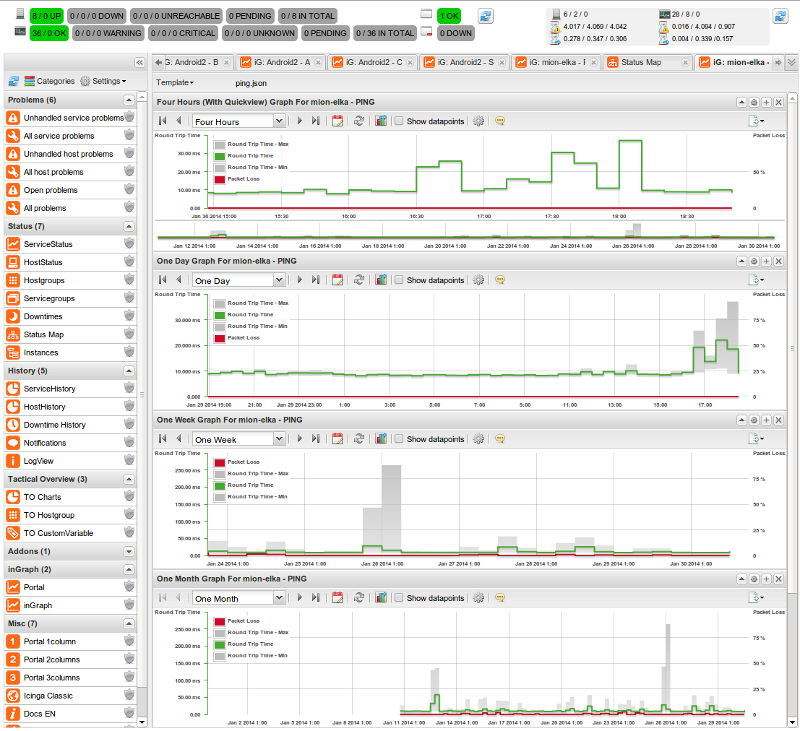
\includegraphics[width=1\textwidth]{img/ingraph.png}
\end{figure}

Interfejs użytkownika dodatku {\em inGraph} został napisany w~językach PHP
oraz JavaScript. Umożliwia on podgląd danych zebranych
i~przetworzonych przez rdzeń dodatku. Interfejs może funkcjonować
zarówno jako niezależny serwis, jak i~integralna część interfejsu
systemu {\em Icinga}. Umożliwia on generację wykresów dla każdego z~urządzeń
oraz dla każdej z~usług. Formaty wykresów, a~także przedziały
agregacji danych, definiowane są w~plikach konfiguracyjnych w~formacie
JSON\footnote{ang. {\em JavaScrip Object Notation} -- lekki format
  tekstowy wymiany danych komputerowych. Szczegółowo opisany
  w~\cite{www:JSON}.}. Użytkownik po wybraniu usługi lub urządzenia
uzyskuje interaktywny wykres przezentujący dane w~zadanym
okresie. Wszystkie wykresy wygenerowane przez program są w~pełni
konfigurowalne i~edytowalne. Typ prezentowanych danych jest
uzależniony od rozmiaru przedziału czasu, w~którym generowany jest
wykres.

Jeśli okno czasu jest odpowiednio małe, na wykresie zostaną
przedstawione dane dokładne. W~sytuacji, gdy nie jest możliwe
przedstawienie danych dokładnych, ze względu na rozmiar zadanego
okresu czasu, dane są agregowane w~przedziały, a~na wykresie
udostępniana jest wartość minimalna, maksymalna oraz średnia dla
danego przedziału agregacji danych. Przykładowe wykresy wygenerowane
przy pomocy dodatku {\em inGraph} przedstawia
rys.~\ref{fig:inGraph}. Szczególną uwagę warto zwrócić na szare pola
reprezentujące minimum oraz maksimum w~danym przedziale.


\section[Dodatek NSCA][Dodatek NSCA]{Dodatek NSCA}
\label{sec:NSCA}

{\em NSCA} - Nagios Service Check Acceptor jest to dodatek do systemów
monitorujących z~rodziny Nagios, więc również systemu {\em Icinga}. Pozwala
on na wykorzystanie mechanizmów pasywnego monitorowania z~systemu
innego niż ten, na którym uruchomione jest oprogramowanie
monitorujące. Program ten został napisany w~całości w~języku~C
i~wydany na licencji pozwalającej na wgląd do kodu
źródłowego. Wykorzystuje on plik komend zewnętrznych (patrz
rozdz.~\ref{sec:IcingaCore}) i~nie integruje się z~rdzeniem
monitorującym. Dzięki temu możliwe jest jego wykorzystanie go w~wielu
konfiguracjach bez konieczności ingerencji w~system monitorujący.

Schemat działania systemu wykorzystującego dodatek {\em NSCA}
został przedstawiony na rys.~\ref{fig:nsca}. Implementacja dodatku
składa się z~dwóch modułów:

\begin{figure}[ht]
  \caption{Schemat działania dodatku NSCA.}
  \label{fig:nsca}
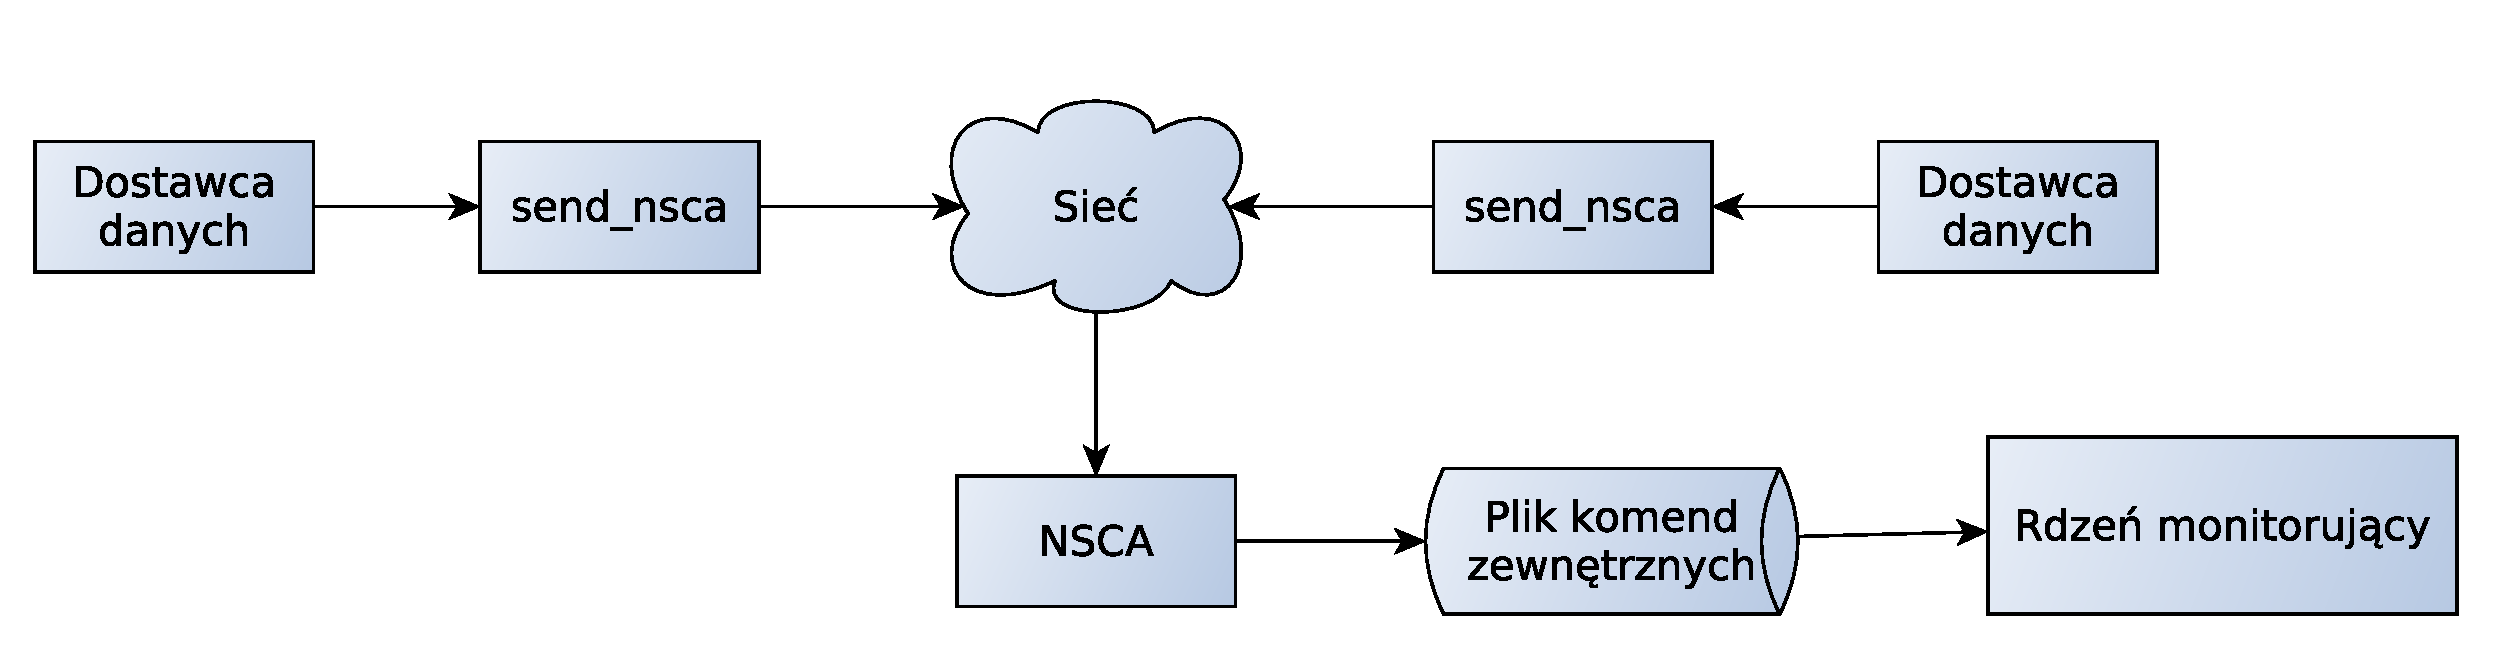
\includegraphics[width=1\textwidth]{img/nsca}
\end{figure}

\begin{itemize}
\item moduł wysyłający (send\_nsca) służący do wysyłania wyników
  sprawdzeń z~monitorującego systemu do centralnego serwera, na którym
  umieszczony jest rdzeń systemu monitorującego odpowiedzialny za
  przetwarzanie wyników sprawdzeń,
\item moduł odbierający (nsca) służący do odbierania wyników sprawdzeń
  od klientów i~dostarczaniu ich do pliku komend zewnętrznych danego
  systemu monitorującego (patrz rozdz.~\ref{sec:IcingaCore}).
\end{itemize}

\subsubsection[send\_nsca][send\_nsca]{send\_nsca}
\label{subsubsec:modulWysylajacy}

Ta część dodatku jest cyklicznie uruchamiana na systemie, na którym
funkcjonuje jakiś mechanizm sprawdzający, który wykonuje sprawdzenia
stanu parametru lub usługi. Mechanizm sprawdzający (np. skrypt
uruchamiany co 10 minut) wykonuje sprawdzenie aktualnego stanu usługi,
a~następnie przekazuje go na standardowe wejście programu
wysyłającego (send\_nsca). Moduł wysyłający, po uruchomieniu
odczytuje ustawienia z~pliku konfiguracyjnego, a~następnie próbuje
połączyć się z~serwerem ({\em NSCA}) używając protokołu TCP. Po udanej
próbie połączenia otrzymuje pakiet inicjujący, który zawiera:

\begin{description}
\item[wektor inicjujący] --- wygenerowany przez serwer pseudolosowy ciąg
  znaków konieczny do inicjalizacji algorytmu kryptograficznego,
\item[stempel czasu] --- czas odczytany przez serwer w~chwili nadejścia
  połączenia od klienta.
\end{description} 

Po otrzymaniu pakietu inicjującego moduł wysyłający rozpoczyna
czytanie danych ze~standardowego wejścia. Wszystkie dane wejściowe
muszą być odpowiednio sformatowane: poszczególne pola informacyjne
muszą być rozdzielone pojedynczą tabulacją, a~cały rezultat pomiaru
zakończony znakiem nowej linii. Sprawdzenia dotyczące urządzenia
powinny zawierać następujące pola:

\begin{description}
\item[nazwa urządzenia] --- krótka nazwa urządzenia, którego stan jest
  przekazywany,
\item[stan] --- numerycznie wyrażony kod stanu urządzenia,
\item[odczyt] --- dodatkowe wartości odczytów opisujące stan
  urządzenia w~ formacie zgodnym z~formatem danych przekazywanych
  przez wtyczki (patrz rozdz.~\ref{sec:IcingaCore}).
\end{description}

Natomiast wpisy dotyczące usług powinny zawierać następujące pola:

\begin{description}
\item[nazwa urządzenia] --- krótka nazwa urządzenia, na którym uruchomiona
  jest usługa,
\item[opis usługi] --- nazwa usługi danego urządzenia, której dotyczy wpis
\item[stan] --- numerycznie wyrażony kod stanu usługi,
\item[odczyt] --- dodatkowe wartości odczytów opisujące stan usługi
  w~formacie zgodnym z~formatem danych przekazywanych przez wtyczki
  (patrz rozdz.~\ref{sec:IcingaCore}).
\end{description}

Łatwo zauważyć, że żadne z~pól wpisu dziennika nie zawiera stempla
czasu wymaganego przez rdzeń sprawdzający przy zapamiętywaniu odczytu
pasywnego. Dzieje się tak, gdyż program {\em NSCA} posiada zdefiniowaną
własną politykę określania czasu wykonania sprawdzenia. Do każdego
pakietu zawierającego wpis dziennika dodawany jest stempel czasu
otrzymany w~pakiecie inicjującym od modułu odbierającego. Właściwy
stempel czasu, który trafia do rdzenia monitorującego nadawany jest
natomiast przez moduł odbierający. Oznacza to przekłamania czasu
pomiary, przy próbie transmisji danych historycznych, zgromadzonych na
skutek np. utraty łączności.

Kolejnym krokiem działania modułu jest obliczenie cyklicznego kodu
nadmiarowego CRC32 dla danego pakietu. Po dołączeniu obliczonego kodu
do pakietu pakiet jest szyfrowany. Algorytm kryptograficzny stosowany
do szyfrowania pakietów został wcześniej zainicjalizowany wektorem
pseudolosowych danych odebranych w~pakiecie inicjalizacyjnym od modułu
odbierającego. Po zaszyfrowaniu dane są wysyłane, a~moduł wysyłający,
bez oczekiwania na potwierdzenie przetworzenia przez serwer,
rozpoczyna przetwarzanie kolejnej porcji danych. Opis przetwarzania
pakietu po stronie serwera {\em NSCA} został opisany dalej w~tym rozdziale.

\subsubsection[Moduł odbierający][Moduł odbierający]{Moduł odbierający}

Demon, który stanowi moduł odbierający funkcjonuje na tym samym
systemie operacyjnym, na którym znajduje się rdzeń systemu
monitorującego. Ta część odpowiedzialna jest za odbieranie danych od
klientów i~przekazywanie ich do rdzenia programu monitorującego. Moduł
ten może pracować w~jednym z~poniższych trybów:

\begin{description}
\item[samodzielny demon jednoprocesowy] --- uruchomiony w~tle demon, który
  nasłuchuje na przychodzące połączenia od klientów i~po nadejściu
  połączenia jest ono obsługiwane przy użyciu jednego procesu z~jednym
  wątkiem,
\item[samodzielny demon wieloprocesowy] --- uruchomiony w~tle demon,
  którego proces główny nasłuchuje na nadejście połączeń od klientów,
  gdy takie połączenie nadejdzie proces jest duplikowany i~każdy
  z~klientów obsługiwany jest w~innym procesie potomnym,
\item[demon zintegrowany z~inetd] --- w~systemie uruchomiony jest demon
  inetd, który nasłuchuje na połączenia od klientów na konkretnym
  gnieździe, a~gdy nadejdzie połączenie od klienta uruchamiany jest
  proces demona {\em NSCA}, który obsługuje nowe połączenie i~kończy się
  wraz z~zakończeniem obsługi klienta.
\end{description}

Niezależnie od trybu pracy, do przekazywania odebranych od zdalnego
systemu danych do rdzenia monitorującego używany jest mechanizm
pasywnego monitorowania dostępny w~systemach z~rodziny Nagios. Aby
możliwe było wykorzystanie tego mechanizmu do przekazania danych z
innych urządzeń konieczne jest zapewnienie demonowi {\em NSCA} dostępu do
pliku zewnętrznych komend systemu monitorującego (patrz
rozdz.~\ref{sec:IcingaCore}). Ponieważ plik ten jest potokiem
nazwanym, chroniony jest on przez Uniksowy system uprawnień
użytkowników. Zapewnienie dostępu do takiego bytu może się odbyć na
dwa sposoby. Pierwszym, polecanym przez twórców systemów
monitorujących, jest uruchamianie demona {\em NSCA} jako procesu tego samego
użytkownika co proces rdzenia systemu monitorującego. Drugim sposobem
jest modyfikacja praw dostępu do omawianego pliku, tak aby umożliwić
dostęp użytkownikowi, z~którego uprawnieniami uruchomiony jest demon
{\em NSCA}. Przy zastosowaniu drugiego rozwiązania zalecana jest szczególna
ostrożność, gdyż dostęp do pliku komend zewnętrznych daje bardzo duże
możliwości ingerencji w~system monitorujący.

Komunikacja modułu odbierającego z~klientem rozpoczyna się od
nadejścia połączenia od klienta. Gdy moduł odbierający otrzyma nowe
połączenie zostanie wysłany pakiet inicjalizujący, którego zawartość
została opisana już wcześniej w~tym rozdziale. Po przesłaniu pakietu
inicjalizującego połączenie, moduł odbierający oczekuje na dane od
klienta. Każdy wynik sprawdzenia przesyłany jest przy użyciu pakietu
o~poniższych polach:

\begin{description}
\item[wersja protokołu] ---  aktualnie używana wersja protokołu komunikacyjnego,
\item[kod CRC32] ---  kod CRC32 bieżącego pakietu,
\item[stempel czasu] --- stempel czasu pochodzący z~pakietu
  inicjalizującego przesłanego klientowi,
\item[kod statusu] --- kod stanu usługi/hosta powiązany z~przesyłanym wpisem
\item[nazwa hosta] --- nazwa urządzenia, które podlegał sprawdzeniu. Nie jest
  konieczne aby było to to samo urządzenie, który dostarcza dane,
\item[opis usługi] --- nazwa usługi, która podlegała sprawdzeniu lub pusty
  napis jeśli sprawdzenie dotyczy urządzenia,
\item[wynik sprawdzenia] --- napis wygenerowany przez wtyczkę, która
  dokonywała sprawdzenia, zawierający dodatkowe dane na temat stanu
  urządzenia lub usługi.
\end{description}

Pakiety są zaszyfrowane z~użyciem algorytmu oraz klucza symetrycznego
pochodzącego z~pliku konfiguracyjnego demona {\em NSCA}. Po odebraniu
spodziewanej ilości danych (wszystkie pakiety mają taką samą długość
wynikającą z~rozmiaru struktury używanej w~programie), następuje próba
odszyfrowania odebranych danych. Sprawdzenie poprawności odebranych
danych i~jednocześnie weryfikacja uprawnień odbywa się poprzez
kontrolę zawartości pola CRC32. Jeśli wartość znajdująca się w~tym
polu zgadza się z~wartością wyliczoną dla otrzymanych danych, to
pakiet jest przyjmowany, w~przeciwnym zaś razie pakiet zostanie
odrzucony bez powiadamiania o~tym jego nadawcy. Dalsze przetwarzanie
otrzymanego pakietu rozpoczyna się od porównania bieżącego stempla
czasu z~tym pochodzącym z~odebranego pakietu. Jeśli różnica pomiędzy
nimi jest zbyt duża, dane zostają odrzucone. Ostatnią czynnością
wykonywaną przez moduł odbierający jest zapisanie odebranego wpisu do
pliku komend zewnętrznych systemu monitorującego.

Warto wspomnieć, że stempel czasu przesłany przez klienta nie jest
dostarczany do jądra monitorującego. Służy on jedynie określeniu
odstępu czasu od inicjalizacji sesji do chwili otrzymania wiadomości
i~podjęciu decyzji o~przyjęciu, bądź odrzuceniu pakietu. Do systemu
monitorującego trafia natomiast bieżący stempel czasu serwera, na
którym uruchomiony jest moduł odbierający i~jądro systemu
monitorującego. Do generacji stempla czasu wykorzystywany jest czas
uniwersalny. W~związku z~powyższym dodatek {\em NSCA} nie umożliwia
synchronizacji danych historycznych. Wszystkie dane, które nadejdą są
traktowane tak, jakby pomiary były wykonane właśnie w~tej chwili.

Istotną może się również okazać informacja, iż protokół komunikacyjny
nie przewiduje przesyłania ACK\footnote {ang. {\em Acknowledgement} --
  pozytywne potwierdzenie, powszechnie przyjęta nazwa komunikatu
  potwierdzającego przyjęcie i~przetworzenie danych przez aplikację.},
bądź też NACK\footnote{ang. {\em Negative Acknowledgement} --
  potwierdzenie negatywne, powszechnie przyjęta nazwa komunikatu
  oznaczająca odmowę przyjęcia lub przetworzenia odebranych
  danych.}. Moduł wysyłający ma zatem pewność, iż wysłane przez niego
dane zostaną dostarczone, gdyż używany jest protokół TCP.  Nie ma
jednak żadnej gwarancji ani informacji, że dane przesłane do modułu
odbierającego zostaną dostarczone do rdzenia systemu monitorującego.

Bezpieczeństwo monitorowania z~użyciem dodatku {\em NSCA} opiera się na
kryptografii symetrycznej oraz cyklicznym kodzie nadmiarowym CRC32
(wielomian: 0xEDB88320). Wiadomość inicjująca połączenie jest
nieszyfrowana. Natomiast każda wiadomość zawierająca dane pomiarowe
jest zaszyfrowana algorytmem wybranym podczas konfiguracji
systemu. Dodatek {\em NSCA} korzysta z~biblioteki
{\em libmcrypt}\footnote{Szczegółowy opis biblioteki jak i~dostępnych w~niej
  algorytmów można znaleźć w~\cite{www:libmcrypt}.} i~umożliwia użycie
jednego spośród wielu algorytmów kryptografii symetrycznej, które
zostały w~niej zaimplementowane. Użytkownik posiada jedynie możliwość
wyboru stosowanego algorytmu, natomiast jako tryb pracy stosowany jest
tryb sprzężenia zwrotnego szyfrogramu (CFB --- ang. {\em Cipher
  Feedback}). Tryb ten wymaga zawsze inicjalizacji zarówno kodera jak
i~dekodera tym samym wektorem początkowym, który w~przypadku tego
protokołu, jest przesyłany przez serwer w~pakiecie inicjującym.

Wszystkie algorytmy symetryczne do prawidłowego działania wymagają,
aby komunikujące się strony współdzieliły pewien sekret jakim jest
klucz używany do szyfrowania. Ujawnienie klucza symetrycznego wiąże
się z~kompromitacją całego systemu kryptograficznego. W~dodatku {\em NSCA}
klucz ten uzyskiwany jest z~hasła, które musi być zapisane przez
administratora systemu w~pliku konfiguracyjnym zarówno części
odbierającej, jak i~wysyłającej. Oczywistym jest, iż poza
współdzieleniem klucza, wszystkie komunikujące się węzły muszą używać
tego samego algorytmu kryptograficznego.

Algorytmy szyfrowania zapewniają tajność przesyłanej wiadomości,
jednak w~przypadku systemu monitorowania potrzebne jest również
zapewnienie integralności. Integralność w~dodatku {\em NSCA} zapewniana jest
poprzez cykliczny kod nadmiarowy CRC32. Przed zaszyfrowaniem
wiadomości obliczany jest jej kod CRC, który jest dołączany do
wiadomości. Następnie wiadomość jest szyfrowana i~przesyłana do
serwera {\em NSCA}. Po odebraniu wiadomości jest ona odszyfrowywana
i~następuje weryfikacja kodu CRC. Jeśli weryfikacja się nie powiedzie
pakiet jest oznaczany jako dane z~naruszoną integralnością
i~w~konsekwencji odrzucany bez powiadomienia o~tym
klienta. W~szczególności, taka sytuacja może się zdarzyć, gdy klient
używa innego algorytmu kryptograficznego lub klucza. Pakiety, których
integralność nie zostanie pozytywnie zweryfikowana są odrzucane.

Model bezpieczeństwa zastosowany w~dodatku {\em NSCA} ma kilka wad. Warto
przypomnieć, iż wszystkie ustawienia zarówno modułu wysyłającego jak
i~odbierającego przechowywane są w~plikach na dyskach odpowiednich
urządzeń. Pliki te zawierają również klucze symetryczne, które są
stosowane w~całym systemie. Oznacza to, iż uzyskanie dostępu typu
odczyt do takiego pliku powoduje utratę tajności danych przesyłanych
w~całym systemie. Ponadto przyjęty model bezpieczeństwa, nie zawiera
żadnej weryfikacji danych pochodzących od klientów. Oznacza to, że
każdy klient może przesłać wpisy dziennika, udające wpisy pochodzące
od zupełnie innych klientów. W~szczególności, jeśli atakujący uzyska
klucz symetryczny, to nie tylko będzie mógł odczytywać informacje
o~danych przesyłanych od klientów, lecz także podszywać się pod
klientów i~przesyłać fałszywe wpisy. Taka luka może być wykorzystana
przy ataku na jakąś usługę lub urządzenie. Atakujący rozpoczyna atak,
po czym przechwytuje pakiety z~wpisami dziennika, które mogą świadczyć
o~rozpoczęciu ataku i~w~zamian przesyła do serwera fałszywe pakiety
informujące, że wszystkie usługi pracują normalnie.

\section[Konfiguracje rozproszone][Podstawowe konfiguracje rozproszone]{Podstawowe konfiguracje rozproszone}

Przedstawione w~trakcie tego rozdziału elementy pozwalają na
zbudowanie w~pełni funkcjonalnego hybrydowego systemu
monitorowania. Schemat takiego systemu został przedstawiony na
rys.~\ref{fig:icingaBase}.

\begin{figure}[htpb]
  \caption{Schemat podstawowej konfiguracji systemu Icinga.}
  \label{fig:icingaBase}
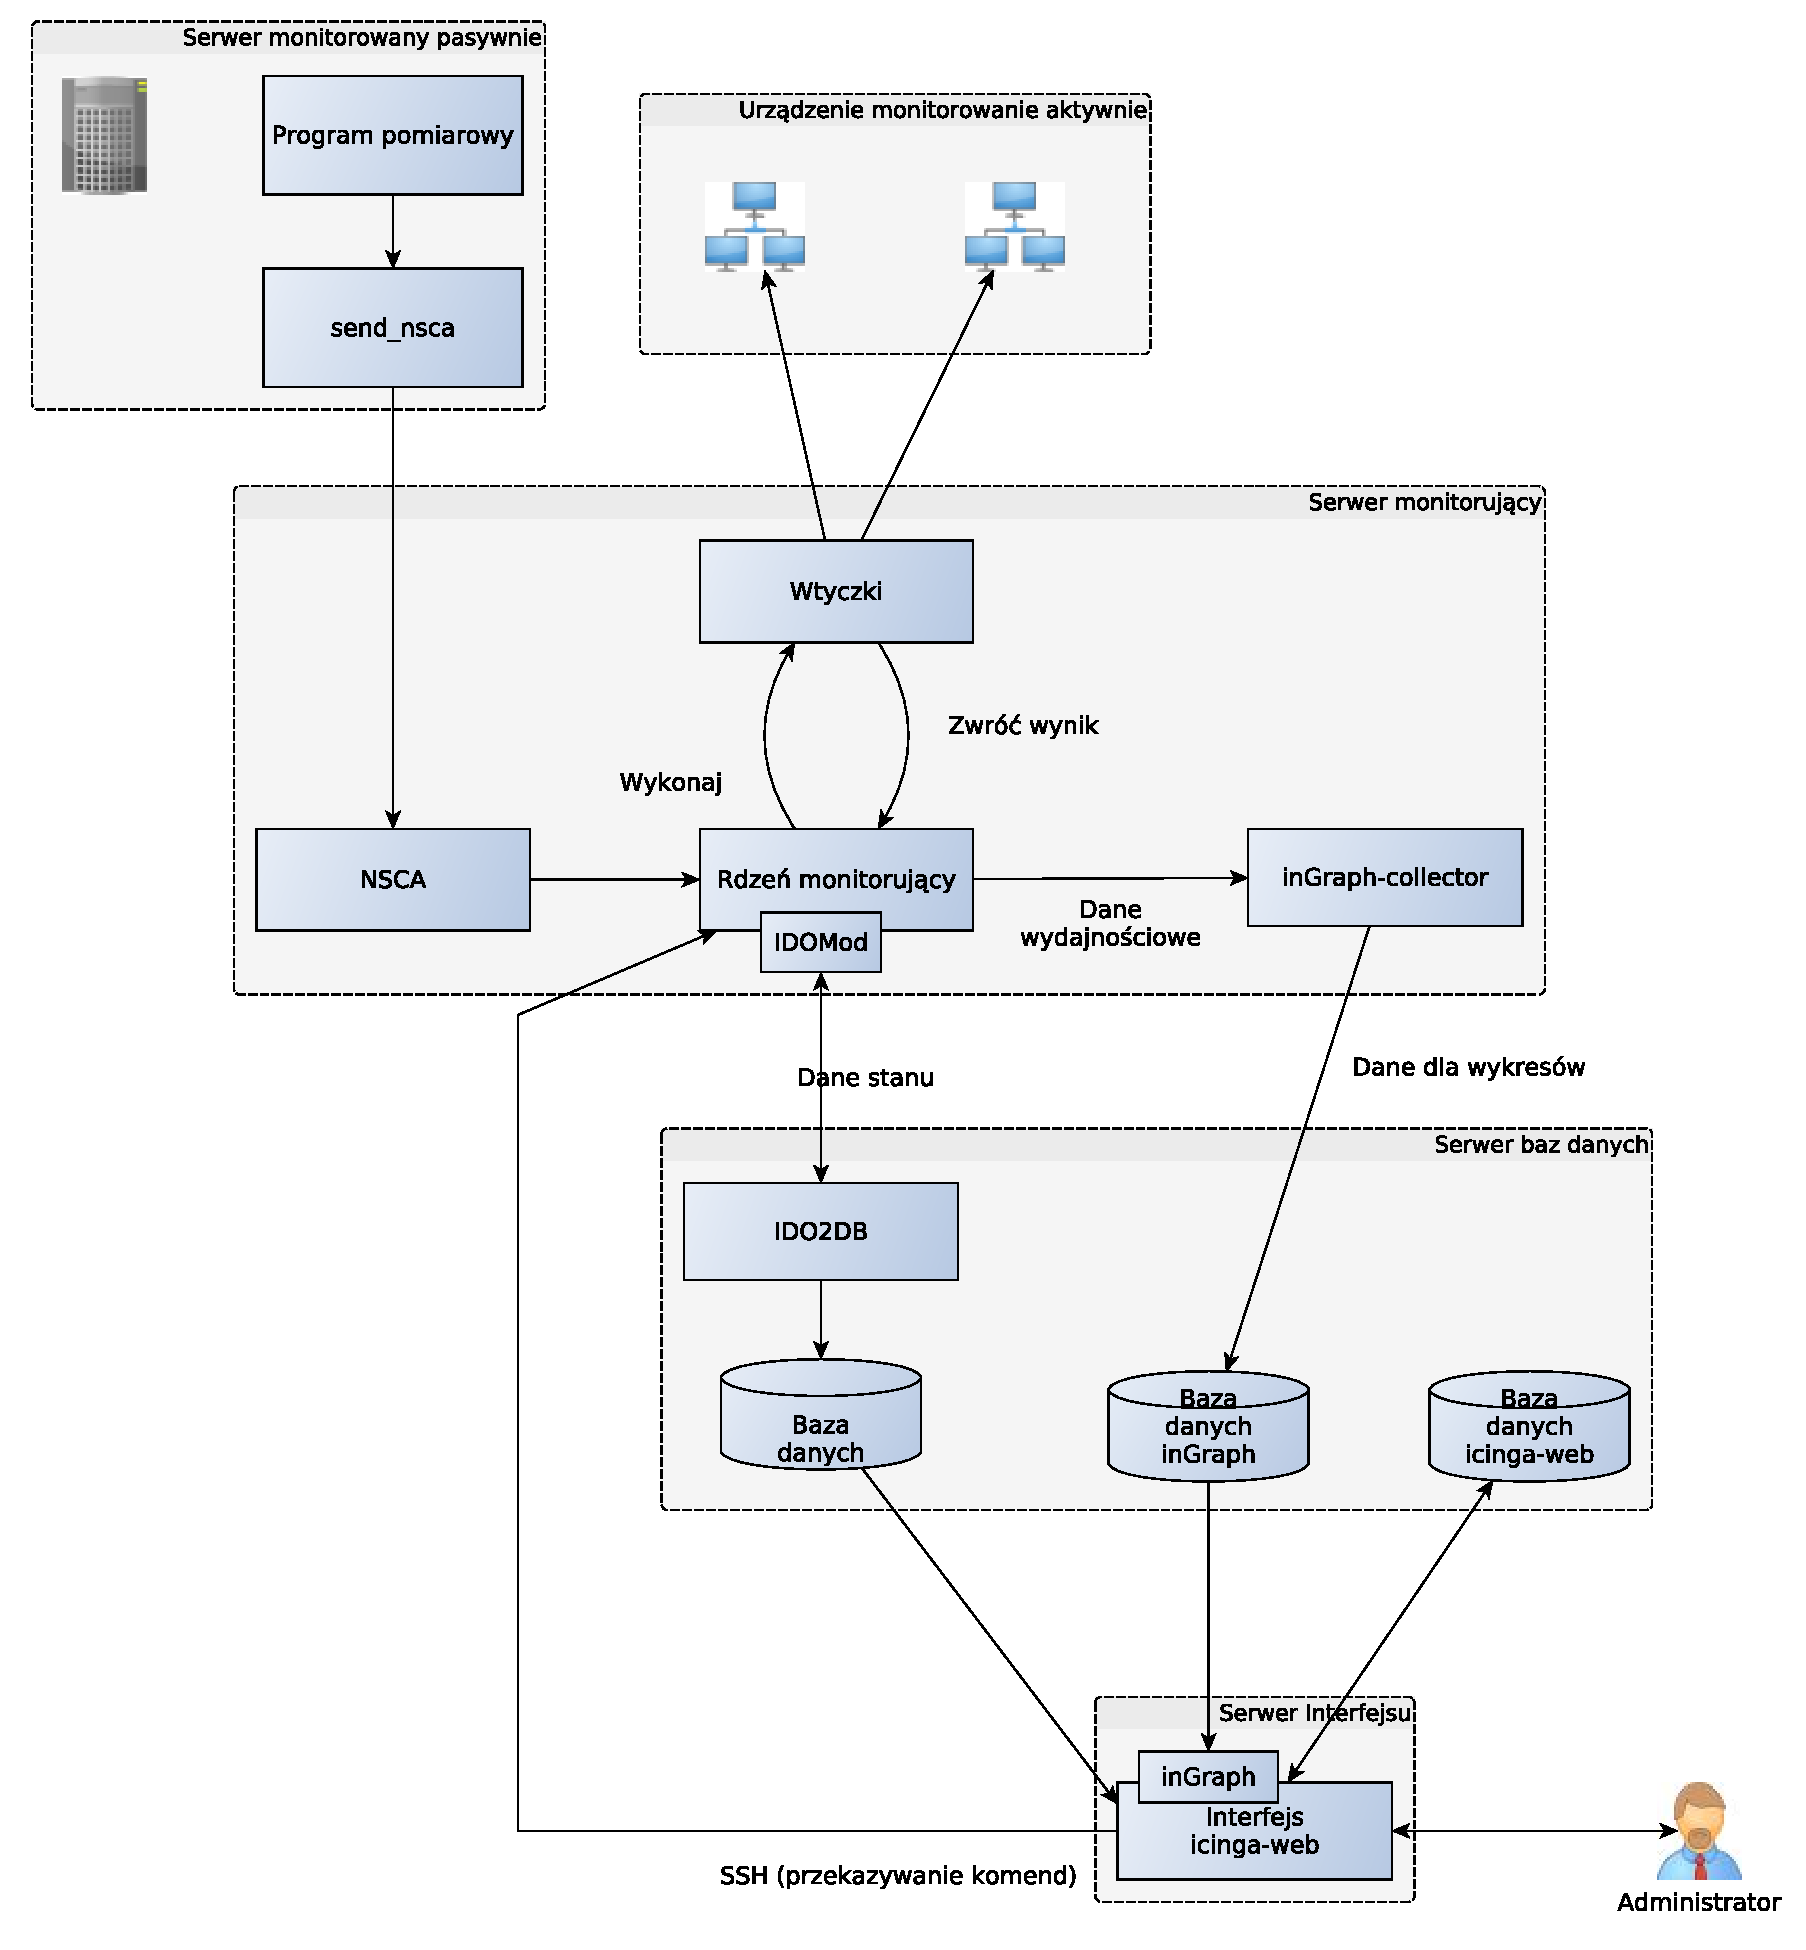
\includegraphics[width=1\textwidth]{img/icingaBase}
\end{figure}

Konfiguracja systemu podzielona jest na kilka części, z~których każda
może znajdować się na innym urządzeniu. Podstawowym elementem systemu
jest serwer monitorujący. Zawiera on przede wszystkim rdzeń
monitorujący {\em Icinga} oraz wtyczki niezbędne do monitorowania
infrastruktury IT. Aby umożliwić monitorowanie urządzeń w~sposób
pasywny na tym samym urządzeniu umieszczony może być program {\em NSCA},
który będzie przekazywał dane pochodzące z~urządzeń monitorowanych
pasywnie do rdzenia poprzez plik komend zewnętrznych. Ponadto na tym
samym serwerze musi znajdować się
{\em ingraph-collector}\footnote{Oczywiście można zrezygnować z tego
  dodatku, jednak uniemożliwi to analizę danych historycznych oraz
  generację wykresów.}. Demon ten uzyskuje dane poprzez eksportowane
przez rdzeń monitorujący pliki z~danymi wydajnościowymi więc nie jest
możliwe umieszczenie go na innym urządzeniu.

Kolejnym elementem systemu jest serwer baz danych. Zawiera on trzy
bazy danych: systemu {\em Icinga}, dodatku {\em inGraph} oraz interfejsu
graficznego. Baza danych systemu {\em Icinga} wypełniana jest poprzez
komponent {\em IDOUtils}, który umieszcza tam dane pochodzące z~rdzenia
monitorującego. Baza ta jest niezbędna do prawidłowego funkcjonowania
interfejsu graficznego, gdyż jest ona dla niego źródłem danych
o~stanie infrastruktury. Baza danych dodatku {\em inGraph} wypełniana jest
przez program {\em ingraph-collector} na podstawie danych wydajnościowych
otrzymanych od rdzenia. W~bazie tej przechowywane są wstępnie
przetworzone dane konieczne do generacji wykresów. Trzecia baza danych
zawiera dane konfiguracyjne interfejsu graficznego, aktualny układ
graficzny, konta użytkowników oraz wszystkie inne dane wymagane do
poprawnego działania serwisu. W~prezentowanej konfiguracji wszystkie
bazy danych znalazły się na jednym urządzeniu jednak nie jest to
konieczne. Możliwe jest rozmieszczenie każdej z~baz na innym
urządzeniu. Ponadto bazy te nie są ze sobą w~żaden sposób powiązane
i~każda z~nich może posiadać własny format.

Ostatnim elementem systemu jest serwer interfejsu
graficznego. Znajduje się na nim interfejs graficzny icinga-web oraz
zintegrowany z~nim interfejs dodatku {\em inGraph}. Aby umożliwić
funkcjonowanie tego interfejsu, konieczne jest umieszczenie na tym
urządzeniu również serwera HTTP jak na przykład Apache. Serwer ten nie
został ujęty na rysunku, gdyż nie stanowi logicznego elementu systemu
monitorującego. Interfejs graficzny uzyskuje wszystkie niezbędne dane
od serwera baz danych. Pozwala on również administratorowi na
przekazywanie do rdzenia monitorującego komend zmieniających jego
zachowanie. Aby zapewnić taką funkcjonalność, konieczne jest
zapewnienie połączenia SSH pomiędzy serwerem interfejsu graficznego,
a~serwerem monitorującym.

Przedstawiona konfiguracja pozwala na kompleksowe monitorowanie
jednosegmentowej sieci. Znaczna cześć przedsiębiorstw posiada jednak
sieć składającą się z~wielu odrębnych segmentów. Monitorowanie takiej
infrastruktury wymaga modyfikacji przedstawionej
konfiguracji. Najprostszą metodą jest użycie monitorowania pasywnego
dla wszystkich urządzeń nie widocznych z~sieci, w~której pracuje rdzeń
monitorujący. Jest to jednak niewygodne i~niezalecane, gdyż nie
pozwala w~pełni wykorzystać funkcjonalności systemu monitorującego,
a~także utrudnia konfiguracje. Konieczne jest zatem użycie jednej
z~dozwolonych konfiguracji zawierających wiele serwerów
monitorujących. Jedna z~dostępnych konfiguracji wykonanych z~użyciem
narzędzia {\em NSCA} została przedstawiona na rys.~\ref{fig:icingaNSCA}.

\begin{figure}[htpb]
  \caption{Schemat konfiguracji rozproszonej z~instancją centralną.}
  \label{fig:icingaNSCA}
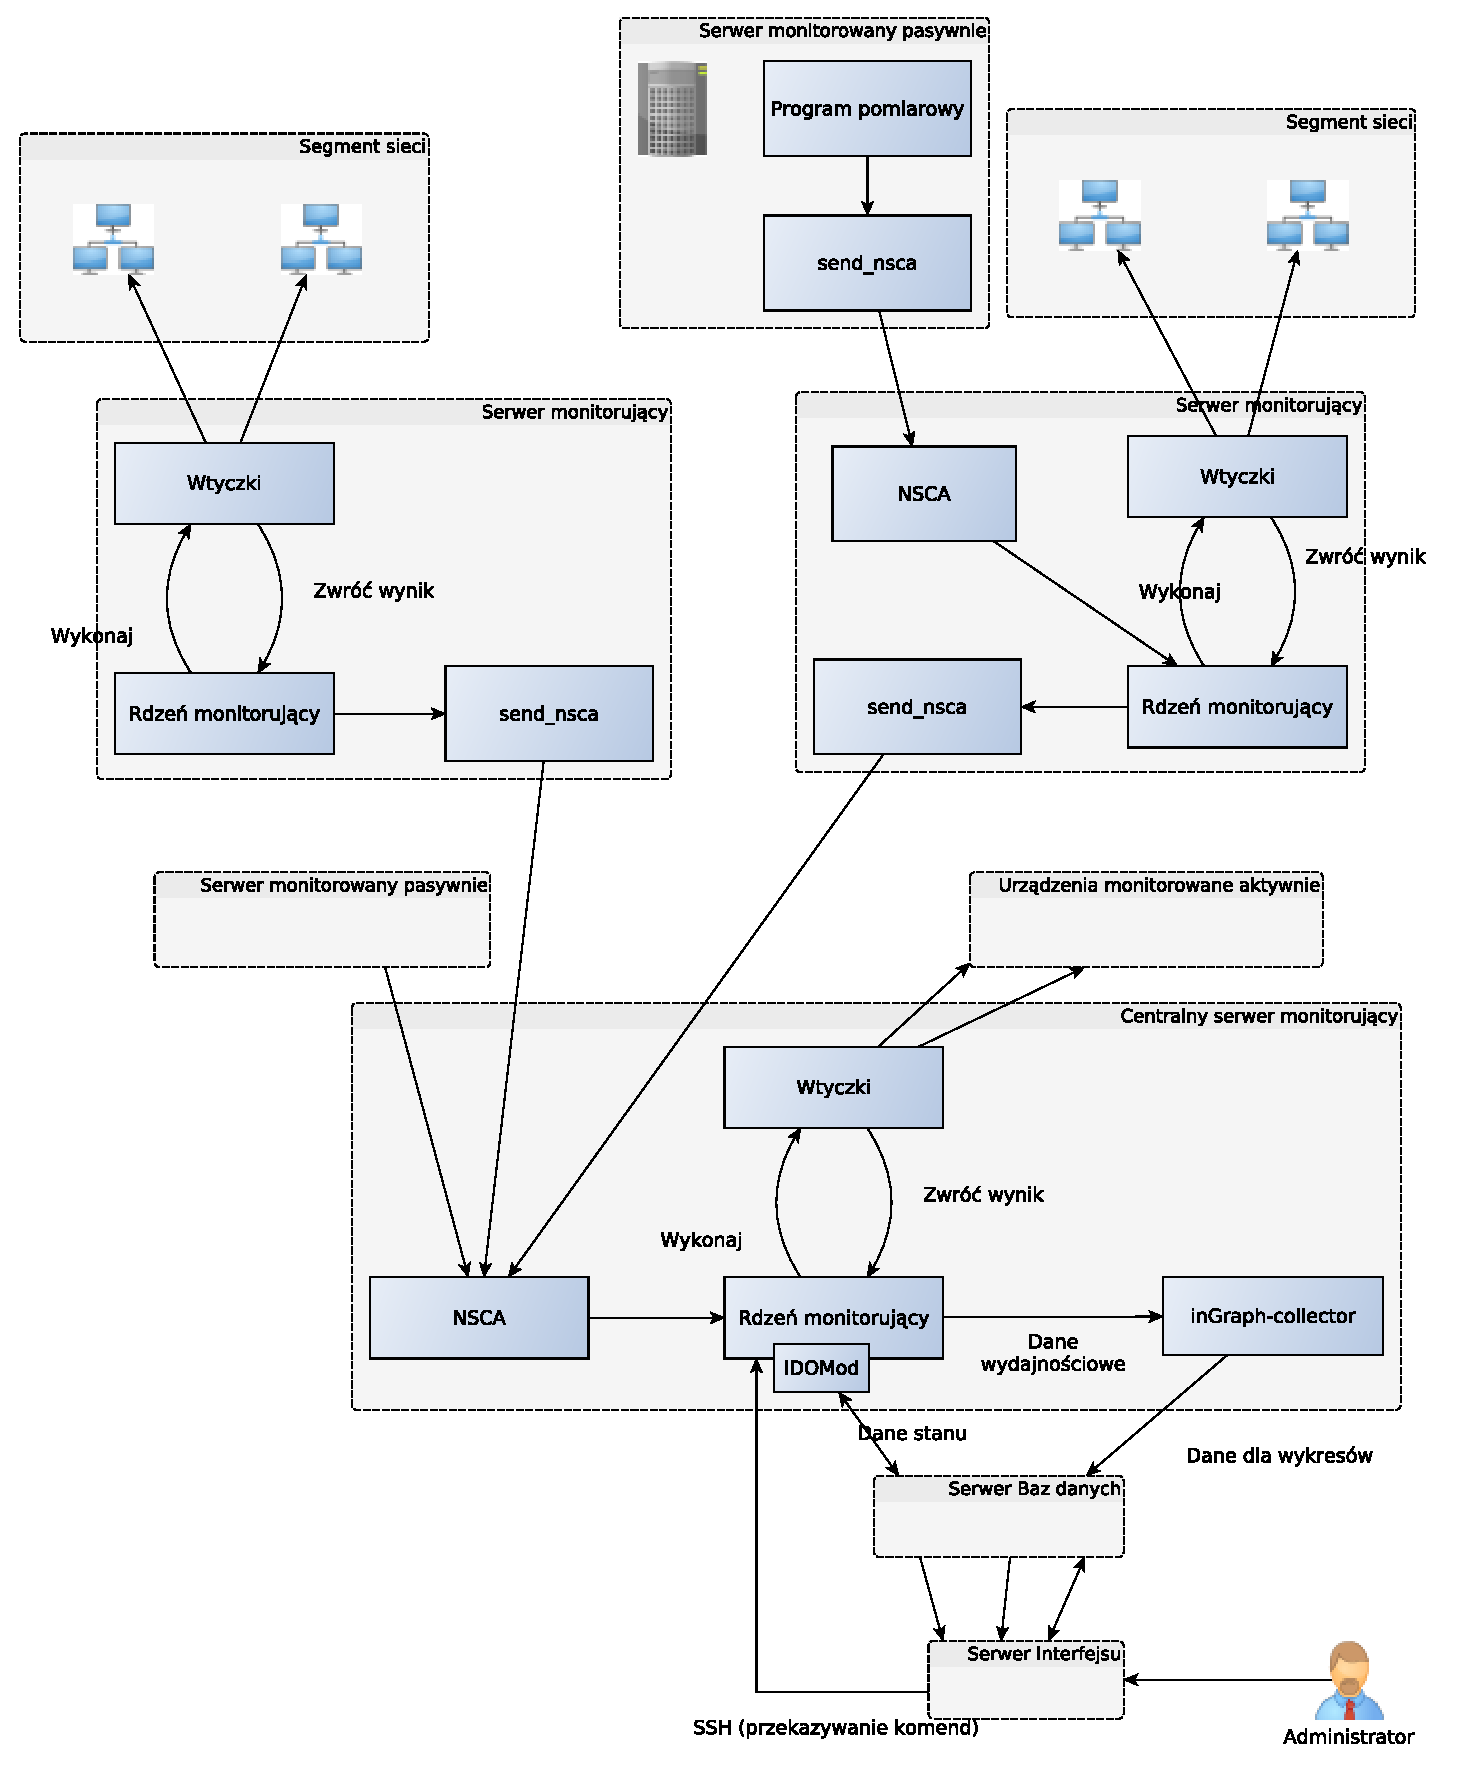
\includegraphics[width=1\textwidth]{img/icingaNSCA}
\end{figure}

Konfiguracja ta zakłada istnienie jednej instancji
centralnej. Instancja ta posiada elementy identyczne jak te, omówione
w~poprzedniej konfiguracji. Istotną różnicą w~stosunku do wcześniej
przedstawionej konfiguracji jest istnienie dodatkowych instancji
podrzędnych. Typowo, co najmniej jedna instancja umieszczona jest
w~każdym odizolowanym segmencie sieci. Każdy taki serwer monitorujący
może monitorować dany segment zarówno w~sposób aktywny, jak
i~pasywny. Istotne jest natomiast, że dane pochodzące z~obu typów
monitorowania są przekazywane do instancji centralnej jako usługi
monitorowane pasywnie. Oznacza to, że z~punktu widzenia instancji
centralnej wszystkie usługi są monitorowane w~sposób pasywny zatem
zajmuje się ona przetwarzaniem wszystkich otrzymanych danych. Jeśli
sieć jest bardzo rozległa może to prowadzić do znacznego obciążenia
serwera centralnego. Z drugiej strony, dzięki wykonywaniu całego
przetwarzania na jednym serwerze możliwa jest bardzo prosta
konfiguracja dodatku {\em inGraph}. Program zbierający dane jest
uruchomiony jedynie na centralnej instancji serwera monitorującego
gdyż to ona przetwarza wszystkie dane.

\begin{figure}[htpb]
\centering
  \caption{Schemat konfiguracji rozproszonej ze~wspólną bazą danych.}
  \label{fig:rozpFull}
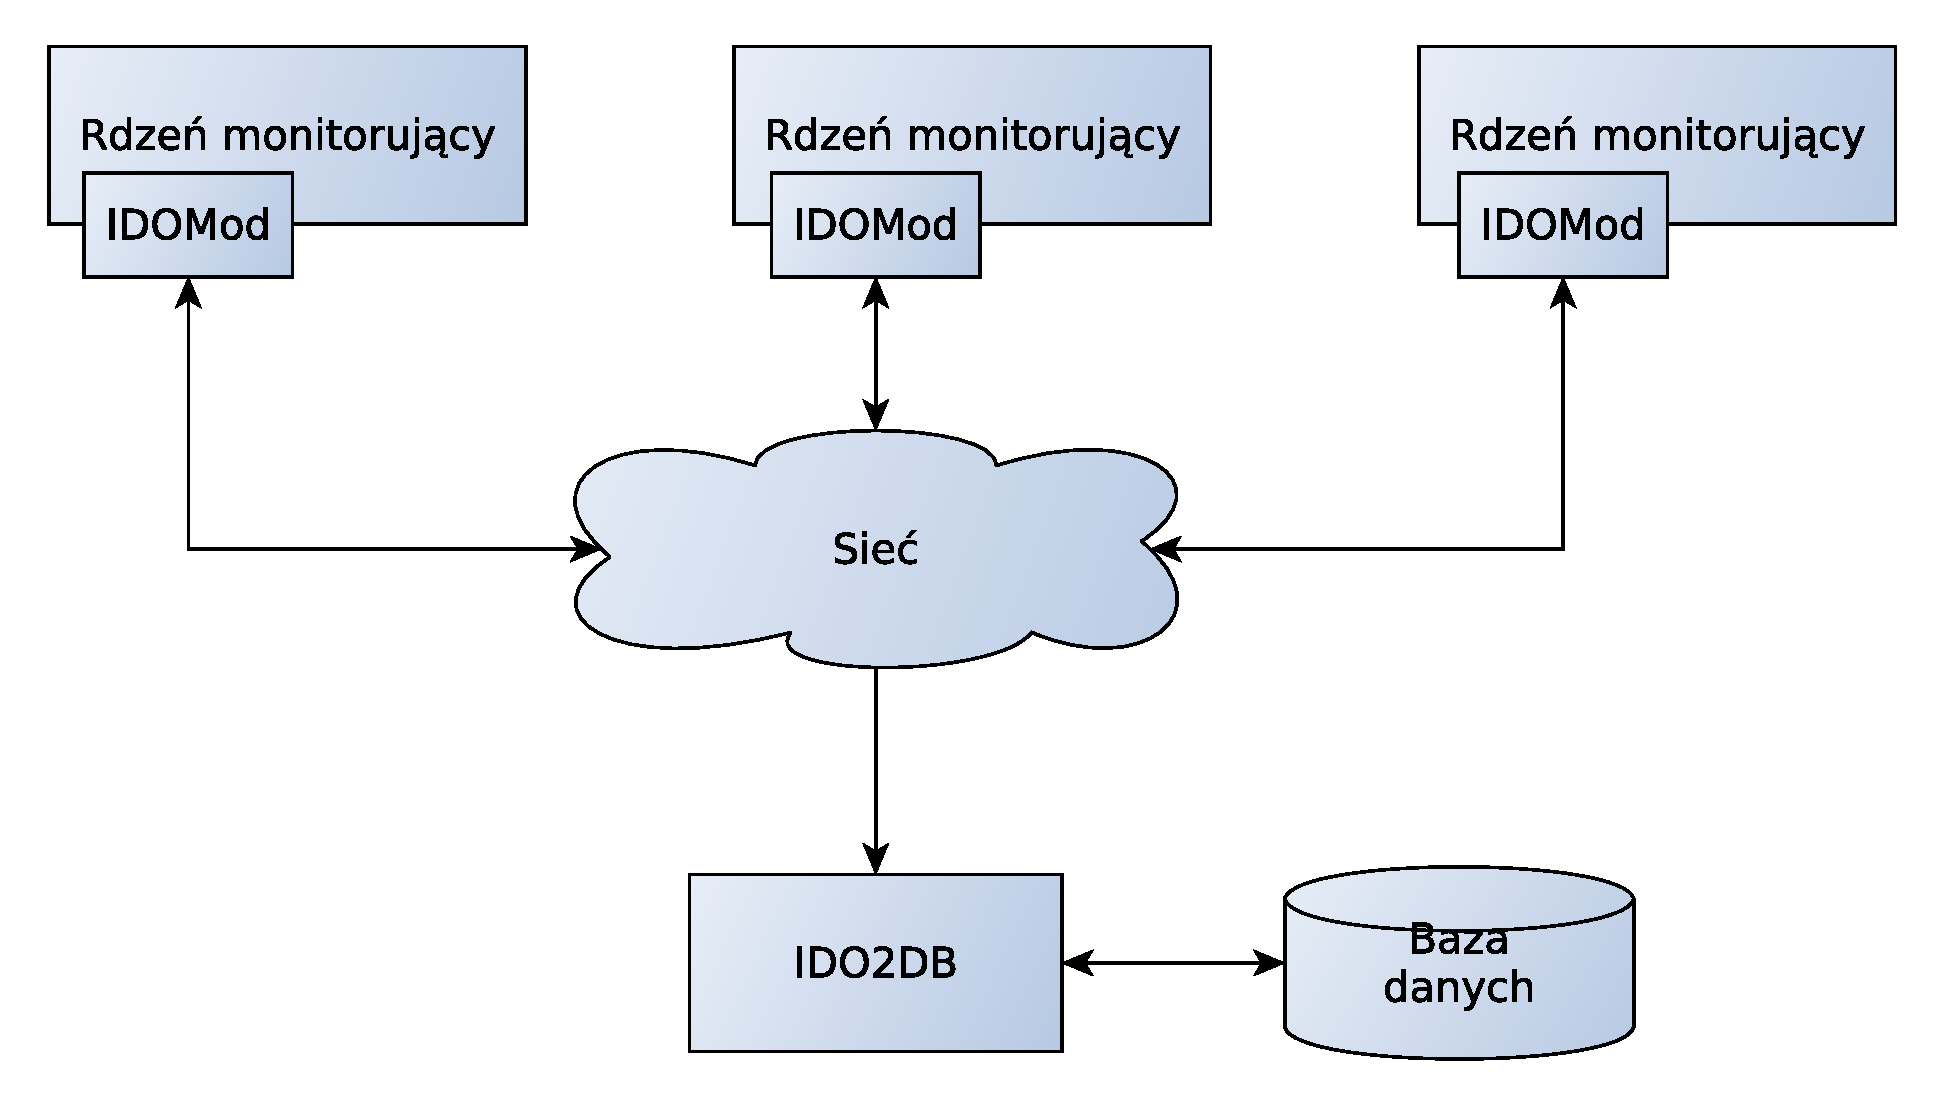
\includegraphics[width=1\textwidth]{img/icingaFull}
\end{figure}

Kolejna z~konfiguracji rozproszonych zakłada wykorzystanie wspólnej
bazy danych. Istnieje wiele instancji systemu monitorującego. Każda
z~nich jest niezależne i~może być nazywana instancją centralną. Każdy
serwer monitoruje wyznaczony segment lub grupę urządzeń. Przetworzone
dane o~stanie usług przekazywane są do wspólnej bazy danych programu
{\em Icinga}. Interfejs graficzny odczytuje te dane z~bazy i~prezentuje
użytkownikowi globalny stan całej infrastruktury. Każdy z~serwerów
odpowiedzialny jest za przetwarzanie danych zebranych z~wyniku
monitorowania wyznaczonej grupy urządzeń. Oznacza to, że każdy
z~rdzeni monitorujących eksportuje na swoim serwerze dane
wydajnościowe pochodzące od monitorowanych urządzeń. Wymusza to
konieczność istnienia na każdym z~serwerów programu {\em ingraph-collector},
który będzie przetwarzał dane od wyznaczonego rdzenia
monitorującego. Należy zwrócić uwagę, że podczas konfiguracji systemu
konieczne jest zadbanie o~unikalne nazwy urządzeń w~ramach całej
infrastruktury, gdyż program ingraph nie posiada żadnych mechanizmów
wykrywania takiej sytuacji i~różne instancje {\em ingraph-collector} mogłyby
wzajemnie nadpisywać gromadzone dane.

Należy zwrócić uwagę, że system {\em Icinga} pozwala na dowolne
zagnieżdżanie przedstawionych konfiguracji. Oznacza to, że możliwe jest
zbudowanie całego drzewa zależności i~przekazywania danych pomiędzy
poszczególnymi instancjami.

Oba rozwiązania posiadają zarówno zalety jak i~wady. Rozwiązanie
z~użyciem dodatku {\em NSCA} zapewnia spójne przetwarzanie danych przez
jedna instancję i~łatwość konfiguracji dodatków wykorzystujących dane
eksportowane przez jądro w~postaci danych wydajnościowych. Niestety
rozwiązanie to generuje znaczące obciążenie instancji centralnej, gdyż
musi ona przetwarzać wszystkie wyniki sprawdzeń. Ponadto należy
przypomnieć, że dodatek {\em NSCA} nie posiada mechanizmu potwierdzającego
przekazanie danych do rdzenia monitorującego. Oznacza to, że w
przypadku niewłaściwej konfiguracji dane mogą być gubione bez
powiadamiania o~tym użytkownika. Rozwiązanie oparte o~wspólną bazę
danych posiada rozproszony mechanizm przetwarzania sprawdzeń jak
i~zdarzeń, dzięki czemu nie występuje w~nim nadmierne obciążenie
jednej z~instancji. Ponadto awaria, dowolnej z~instancji nie powoduje
nigdy braku możliwości monitorowania całej sieci lecz jedynie jej
fragmentu. Niestety w~rozwiązaniu tym konieczna jest bardziej
zaawansowana konfiguracja dodatków korzystających z~danych
wydajnościowych. Wybór konfiguracji zależy zatem silnie od
infrastruktury w~jakiej ma być ona zastosowana, a~także od pozostałych
elementów systemu, jakie będą wykorzystane.


